% Options for packages loaded elsewhere
\PassOptionsToPackage{unicode}{hyperref}
\PassOptionsToPackage{hyphens}{url}
%
\documentclass[
]{book}
\usepackage{lmodern}
\usepackage{amssymb,amsmath}
\usepackage{ifxetex,ifluatex}
\ifnum 0\ifxetex 1\fi\ifluatex 1\fi=0 % if pdftex
  \usepackage[T1]{fontenc}
  \usepackage[utf8]{inputenc}
  \usepackage{textcomp} % provide euro and other symbols
\else % if luatex or xetex
  \usepackage{unicode-math}
  \defaultfontfeatures{Scale=MatchLowercase}
  \defaultfontfeatures[\rmfamily]{Ligatures=TeX,Scale=1}
\fi
% Use upquote if available, for straight quotes in verbatim environments
\IfFileExists{upquote.sty}{\usepackage{upquote}}{}
\IfFileExists{microtype.sty}{% use microtype if available
  \usepackage[]{microtype}
  \UseMicrotypeSet[protrusion]{basicmath} % disable protrusion for tt fonts
}{}
\makeatletter
\@ifundefined{KOMAClassName}{% if non-KOMA class
  \IfFileExists{parskip.sty}{%
    \usepackage{parskip}
  }{% else
    \setlength{\parindent}{0pt}
    \setlength{\parskip}{6pt plus 2pt minus 1pt}}
}{% if KOMA class
  \KOMAoptions{parskip=half}}
\makeatother
\usepackage{xcolor}
\IfFileExists{xurl.sty}{\usepackage{xurl}}{} % add URL line breaks if available
\IfFileExists{bookmark.sty}{\usepackage{bookmark}}{\usepackage{hyperref}}
\hypersetup{
  pdftitle={Prácticas de Ingeniería de Servidores},
  pdfauthor={Alonso Bueno Herrero},
  hidelinks,
  pdfcreator={LaTeX via pandoc}}
\urlstyle{same} % disable monospaced font for URLs
\usepackage{color}
\usepackage{fancyvrb}
\newcommand{\VerbBar}{|}
\newcommand{\VERB}{\Verb[commandchars=\\\{\}]}
\DefineVerbatimEnvironment{Highlighting}{Verbatim}{commandchars=\\\{\}}
% Add ',fontsize=\small' for more characters per line
\usepackage{framed}
\definecolor{shadecolor}{RGB}{248,248,248}
\newenvironment{Shaded}{\begin{snugshade}}{\end{snugshade}}
\newcommand{\AlertTok}[1]{\textcolor[rgb]{0.94,0.16,0.16}{#1}}
\newcommand{\AnnotationTok}[1]{\textcolor[rgb]{0.56,0.35,0.01}{\textbf{\textit{#1}}}}
\newcommand{\AttributeTok}[1]{\textcolor[rgb]{0.77,0.63,0.00}{#1}}
\newcommand{\BaseNTok}[1]{\textcolor[rgb]{0.00,0.00,0.81}{#1}}
\newcommand{\BuiltInTok}[1]{#1}
\newcommand{\CharTok}[1]{\textcolor[rgb]{0.31,0.60,0.02}{#1}}
\newcommand{\CommentTok}[1]{\textcolor[rgb]{0.56,0.35,0.01}{\textit{#1}}}
\newcommand{\CommentVarTok}[1]{\textcolor[rgb]{0.56,0.35,0.01}{\textbf{\textit{#1}}}}
\newcommand{\ConstantTok}[1]{\textcolor[rgb]{0.00,0.00,0.00}{#1}}
\newcommand{\ControlFlowTok}[1]{\textcolor[rgb]{0.13,0.29,0.53}{\textbf{#1}}}
\newcommand{\DataTypeTok}[1]{\textcolor[rgb]{0.13,0.29,0.53}{#1}}
\newcommand{\DecValTok}[1]{\textcolor[rgb]{0.00,0.00,0.81}{#1}}
\newcommand{\DocumentationTok}[1]{\textcolor[rgb]{0.56,0.35,0.01}{\textbf{\textit{#1}}}}
\newcommand{\ErrorTok}[1]{\textcolor[rgb]{0.64,0.00,0.00}{\textbf{#1}}}
\newcommand{\ExtensionTok}[1]{#1}
\newcommand{\FloatTok}[1]{\textcolor[rgb]{0.00,0.00,0.81}{#1}}
\newcommand{\FunctionTok}[1]{\textcolor[rgb]{0.00,0.00,0.00}{#1}}
\newcommand{\ImportTok}[1]{#1}
\newcommand{\InformationTok}[1]{\textcolor[rgb]{0.56,0.35,0.01}{\textbf{\textit{#1}}}}
\newcommand{\KeywordTok}[1]{\textcolor[rgb]{0.13,0.29,0.53}{\textbf{#1}}}
\newcommand{\NormalTok}[1]{#1}
\newcommand{\OperatorTok}[1]{\textcolor[rgb]{0.81,0.36,0.00}{\textbf{#1}}}
\newcommand{\OtherTok}[1]{\textcolor[rgb]{0.56,0.35,0.01}{#1}}
\newcommand{\PreprocessorTok}[1]{\textcolor[rgb]{0.56,0.35,0.01}{\textit{#1}}}
\newcommand{\RegionMarkerTok}[1]{#1}
\newcommand{\SpecialCharTok}[1]{\textcolor[rgb]{0.00,0.00,0.00}{#1}}
\newcommand{\SpecialStringTok}[1]{\textcolor[rgb]{0.31,0.60,0.02}{#1}}
\newcommand{\StringTok}[1]{\textcolor[rgb]{0.31,0.60,0.02}{#1}}
\newcommand{\VariableTok}[1]{\textcolor[rgb]{0.00,0.00,0.00}{#1}}
\newcommand{\VerbatimStringTok}[1]{\textcolor[rgb]{0.31,0.60,0.02}{#1}}
\newcommand{\WarningTok}[1]{\textcolor[rgb]{0.56,0.35,0.01}{\textbf{\textit{#1}}}}
\usepackage{longtable,booktabs}
% Correct order of tables after \paragraph or \subparagraph
\usepackage{etoolbox}
\makeatletter
\patchcmd\longtable{\par}{\if@noskipsec\mbox{}\fi\par}{}{}
\makeatother
% Allow footnotes in longtable head/foot
\IfFileExists{footnotehyper.sty}{\usepackage{footnotehyper}}{\usepackage{footnote}}
\makesavenoteenv{longtable}
\usepackage{graphicx,grffile}
\makeatletter
\def\maxwidth{\ifdim\Gin@nat@width>\linewidth\linewidth\else\Gin@nat@width\fi}
\def\maxheight{\ifdim\Gin@nat@height>\textheight\textheight\else\Gin@nat@height\fi}
\makeatother
% Scale images if necessary, so that they will not overflow the page
% margins by default, and it is still possible to overwrite the defaults
% using explicit options in \includegraphics[width, height, ...]{}
\setkeys{Gin}{width=\maxwidth,height=\maxheight,keepaspectratio}
% Set default figure placement to htbp
\makeatletter
\def\fps@figure{htbp}
\makeatother
\setlength{\emergencystretch}{3em} % prevent overfull lines
\providecommand{\tightlist}{%
  \setlength{\itemsep}{0pt}\setlength{\parskip}{0pt}}
\setcounter{secnumdepth}{5}
\usepackage{booktabs}
\usepackage[]{natbib}
\bibliographystyle{apalike}

\title{Prácticas de Ingeniería de Servidores}
\author{Alonso Bueno Herrero}
\date{Curso 2019-20. Última modificación: 2021-03-24}

\begin{document}
\maketitle

{
\setcounter{tocdepth}{1}
\tableofcontents
}
\hypertarget{p1}{%
\chapter{\texorpdfstring{Instalación de servidores: \textbf{\emph{Ubuntu Server}} y \textbf{\emph{centOS}}}{Instalación de servidores: Ubuntu Server y centOS}}\label{p1}}

\hypertarget{objetivos-de-la-pruxe1ctica}{%
\section{Objetivos de la práctica}\label{objetivos-de-la-pruxe1ctica}}

Objetivos mínimos:

\begin{enumerate}
\def\labelenumi{\arabic{enumi}.}
\tightlist
\item
  Familiarizarse con distintos Sistemas Operativos (SOs) usados en servidores.
\item
  Conocer alternativas comerciales para tener un servidor.
\item
  Configurar unidades de disco RAID y LVM.
\item
  Configurar una red local de máquinas virtuales.
\end{enumerate}

\hypertarget{sesiuxf3n-1-instalaciuxf3n-de-ubuntu-server-y-centos}{%
\section{Sesión 1: Instalación de Ubuntu Server y centOS}\label{sesiuxf3n-1-instalaciuxf3n-de-ubuntu-server-y-centos}}

\hypertarget{conceptos-buxe1sicos}{%
\subsection{Conceptos básicos}\label{conceptos-buxe1sicos}}

Repasamos los siguientes conceptos básicos que conviene conocer antes de iniciar las tareas de esta sesión:

\begin{enumerate}
\def\labelenumi{\arabic{enumi}.}
\item
  Servidor, como un sistema informático que recibe peticiones y da respuestas a las mismas.
\item
  Tecnología de servidores, distinguiendo:

  \begin{enumerate}
  \def\labelenumii{\alph{enumii}.}
  \tightlist
  \item
    \textbf{\emph{Hosting}} dedicado:es una configuración de alojamiento en el que se dedica un servidor a una sola organización o para un solo propósito, como una página web. No escalable.
  \item
    \textbf{\emph{VPS}} (Virtual Private Server), donde varias MV comparten una serie de recursos hardware (Disco Duro, RAM, CPU, \ldots).
  \item
    \textbf{\emph{Serverless}} (servicios en la nube), las aplicaciones montan ahí sus recursos y todas las tareas de administración de sistema están abstraídas para el usuario hasta el punto que él no tiene que preocuparse de las mismas. Es el modelo más actual por su alta capacidad de escalabilidad.
  \end{enumerate}
\item
  Una tecnología de servidores basada en contenedores se caracteriza porque cada uno de estos contenedores se interpreta como una MV, sólo que cada una de esas MV son aplicaciones sobre el SO anfitrión, en tanto en cuanto:

  \begin{itemize}
  \tightlist
  \item
    Los contenedores están (pueden estar) interconectados entre sí,
  \item
    Puedo añadir nuevos contenedores dinámicamente e ir conectándolos a otros que estén en activo (arrancados, funcionando).
  \end{itemize}

  Un ejemplo es un servidor web donde un contenedor C1 contiene el motor web, otro C2 contiene la base de datos y el C3, que contendría el intérprete de peticiones web.
\item
  La tecnología \emph{RAID} surge como solución a la problemática del precio del almacenamiento. Las siglas se refieren a \textbf{\emph{Redundant Array of Independent Disks}} (Almacén Redundante de Discos Independientes). Existen diversos tipos de tecnologías RAID, las más importantes son RAID-0 y RAID-1:

  \begin{enumerate}
  \def\labelenumii{\alph{enumii}.}
  \tightlist
  \item
    \emph{RAID-0}. Un RAID-0 distribuye los datos equitativamente entre dos o más discos (usualmente se ocupa el mismo espacio en dos o más discos) sin información de paridad que proporcione redundancia. Es importante señalar que el RAID 0 no es redundante. Un RAID 0 puede ser creado con discos de diferentes tamaños, pero el espacio de almacenamiento añadido al conjunto estará limitado por el tamaño del disco más pequeño (por ejemplo, si se hace un conjunto dividido con un disco de 450 GB y otro de 100 GB, el tamaño del conjunto resultante será sólo de 200 GB, ya que cada disco aporta 100 GB).
  \item
    Un RAID 1 crea una copia exacta (o espejo) de un conjunto de datos en dos o más discos. Esto resulta útil cuando queremos tener más seguridad desaprovechando capacidad, ya que si perdemos un disco, tenemos el otro con la misma información. Un conjunto RAID 1 sólo puede ser tan grande como el más pequeño de sus discos. Un RAID 1 clásico consiste en dos discos en espejo, lo que incrementa exponencialmente la fiabilidad respecto a un solo disco; es decir, que para que el conjunto falle es necesario que lo hagan todos sus discos.
  \item
    \textbf{Ejercicio} Busca información sobre los tipos de RAID siguientes: RAID-10, RAID-5 y RAID-6.
  \end{enumerate}
\end{enumerate}

\begin{Shaded}
\begin{Highlighting}[]
\NormalTok{knitr}\OperatorTok{::}\KeywordTok{include_graphics}\NormalTok{(}\StringTok{"images/raid0.png"}\NormalTok{)}
\end{Highlighting}
\end{Shaded}

\begin{figure}

{\centering 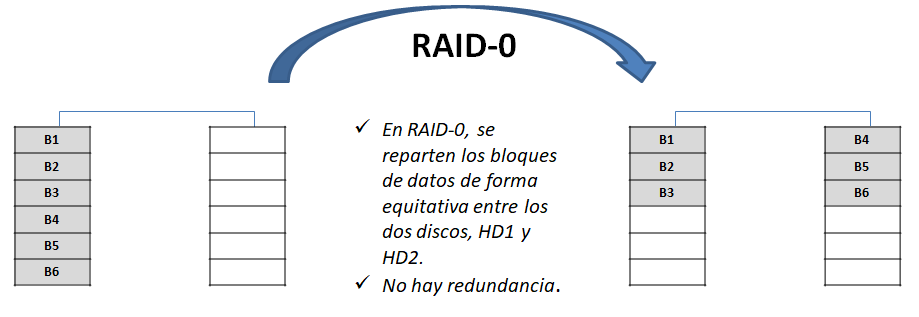
\includegraphics[width=0.9\linewidth]{images/raid0} 

}

\caption{Configuración de RAID-0. Elaboración propia.}\label{fig:rmarkdown}
\end{figure}

\begin{enumerate}
\def\labelenumi{\arabic{enumi}.}
\setcounter{enumi}{4}
\tightlist
\item
  Sistema de archivos

  \begin{enumerate}
  \def\labelenumii{\alph{enumii}.}
  \tightlist
  \item
    Sistema de archivos \emph{ext2}: principales características:

    \begin{itemize}
    \tightlist
    \item
      No admite Journaling
    \item
      Adecuado para tarjetas SD y unidades USB, ya que tiene un alto rendimiento y escritura baja (ya que el registro en diario no está disponible). USB y almacenamiento SD están limitados con ciclos de escritura por lo tanto su mejor ajuste para ellos.
    \item
      Límites: Tamaño de archivo individual de 16 GB a 2 TB.
    \item
      Tamaño del sistema de archivos de 2TB a 32TB.
    \end{itemize}
  \item
    Sistema de archivos ext4

    \begin{itemize}
    \tightlist
    \item
      Soporta Journaling
    \item
      Muchas de las nuevas características introducidas. Extents, Compatibilidad con versiones anteriores, Pre-asignación persistente, Asignación diferida, Número ilimitado de subdirectorios, Suma de comprobación del diario, Comprobación FS más rápida, Encriptación transparente.
    \item
      Límites: Tamaño de archivo individual de 16GB a 16TB. Tamaño del sistema de archivos hasta 1EB.
    \item
      No es necesario actualizar el sistema de archivos. Debido a la compatibilidad hacia atrás, ext2, ext3 se puede montar directamente como ext4.
    \end{itemize}
  \end{enumerate}
\end{enumerate}

\hypertarget{proceso-de-instalaciuxf3n-de-ubuntu-server-16.04}{%
\subsection{Proceso de instalación de Ubuntu Server 16.04}\label{proceso-de-instalaciuxf3n-de-ubuntu-server-16.04}}

\hypertarget{sesiuxf3n-2-ampliaciuxf3n-de-capacidad-para-un-usuario-en-el-servidor-centos.}{%
\section{\texorpdfstring{Sesión 2: Ampliación de capacidad para un usuario en el servidor \textbf{\emph{centOS}}.}{Sesión 2: Ampliación de capacidad para un usuario en el servidor centOS.}}\label{sesiuxf3n-2-ampliaciuxf3n-de-capacidad-para-un-usuario-en-el-servidor-centos.}}

En este caso, la idea es que, una vez instalado el servidor de centOS en el disco por defecto que nos crea VirtualBox, añadamos más capacidad a la ``carpeta'' de ese usuario concreto.

Para estas operaciones habrá que tener en cuenta algunas consideraciones y delicadezas de centOS con respecto a Ubuntu. Pero ya las iremos viendo\ldots{}

\hypertarget{contextualizaciuxf3n-del-escenario-profesional}{%
\subsection{Contextualización del escenario profesional}\label{contextualizaciuxf3n-del-escenario-profesional}}

El escenario profesional es el siguiente: En esta ocasión, en la empresa en la que le acaban de contratar tenían adquirido un servidor y su predecesor había realizado la instalación del S.O. CentOS, según le han comentado los compañeros, él solía hacer instalaciones por defecto y luego aplicar scripts de configuración. Sin más información, nuestro jefe nos informa que esa máquina va a alojar unos cursos con vídeos de alta calidad y relativamente largos. Por tanto, viendo la configuración del sistema, prevemos que /var necesitará más espacio, incluso es conveniente asignarle un LV exclusivamente. Para ello, incluiremos un nuevo disco y configuraremos LVM para que /var se monte en el nuevo VL que crearemos para él.

\hypertarget{pasos-previos-instalaciuxf3n-de-centos}{%
\subsection{\texorpdfstring{Pasos previos: instalación de \textbf{\emph{centOS}}}{Pasos previos: instalación de centOS}}\label{pasos-previos-instalaciuxf3n-de-centos}}

\begin{quote}
Recuerda que al instalar centOS hay que crear el usuario con su clave y darle permisos de administrador. Además tienes que establecer contraseña de root para poder hacer todo lo siguiente.
\end{quote}

\hypertarget{procedimiento}{%
\subsection{Procedimiento}\label{procedimiento}}

Pasos a realizar:

\begin{enumerate}
\def\labelenumi{\arabic{enumi}.}
\tightlist
\item
  Una vez hecha la instalación por defecto, y al iniciar sesión en el servidor, se nos proporciona el siguiente \emph{sistema de particiones} sobre el único disco que tenemos, de 8 GB, que le habíamos proporcionado (ver figura \ref{fig:a}).
\end{enumerate}

\begin{figure}

{\centering 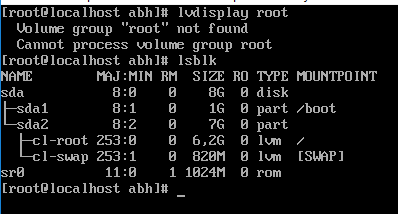
\includegraphics[width=0.6\linewidth]{images/a} 

}

\caption{Situación de particionado del primer disco tras instalar centOS con las opciones por defecto.}\label{fig:a}
\end{figure}

Es decir, que el volumen físico \texttt{sda2}tiene 7GB y en él se ubica el VG llamado \texttt{cl}, donde están los volúmenes lógicos \texttt{root} (de 6,2 GB) y \texttt{swap} (de 820 MB).

\begin{enumerate}
\def\labelenumi{\arabic{enumi}.}
\setcounter{enumi}{1}
\tightlist
\item
  Añadamos el nuevo disco y configurémoslo para que \texttt{/var} tenga ese espacio extra (todo esto tiene detrás un proceso relativamente corto que iremos viendo).
\end{enumerate}

Por ahora, apagamos el ordenador (comando \texttt{poweroff}), añadimos el nuevo disco a nuestra Máquina Virtual y arrancamos. La situación tras añadir el nuevo disco ``físico'' y hacer \texttt{lsblk} es se ve en la figura \ref{fig:b}.

\begin{figure}

{\centering 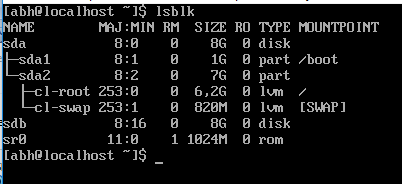
\includegraphics[width=0.6\linewidth]{images/b} 

}

\caption{Situación tras aña}\label{fig:b}
\end{figure}

\begin{enumerate}
\def\labelenumi{\arabic{enumi}.}
\setcounter{enumi}{2}
\tightlist
\item
  Como vemos, aparece el disco \texttt{sdb}, que es el nuevo disco que hemos añadido, pero vemos que no tiene ningún PV (volumen físico) asociado, con lo cual es como si ese espacio lo tuviéramos inútil al completo. Comprobémoslo con la(s) orden(es) de LVM que nos informa(n) de los volúmenes físicos existentes en nuestro sistema: \texttt{pvdisplay} o de forma resumida, \texttt{pvs} (ver figura \ref{fig:c}).
\end{enumerate}

\begin{figure}

{\centering 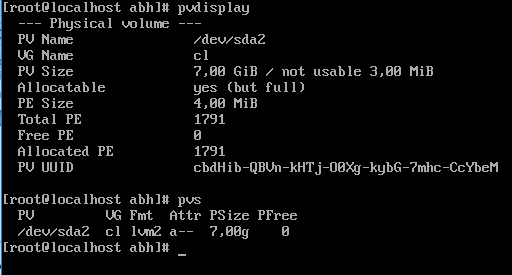
\includegraphics[width=0.6\linewidth]{images/c} 

}

\caption{Mostrando los volúmenes físicos actuales. }\label{fig:c}
\end{figure}

\begin{verbatim}
Y vemos que en efecto no refleja nada sobre el segundo disco creado. 
\end{verbatim}

\begin{enumerate}
\def\labelenumi{\arabic{enumi}.}
\setcounter{enumi}{3}
\tightlist
\item
  Lo primero que vamos a hacer es definir el volumen físico asociado a ese nuevo disco, para ello usaremos el comando \texttt{pvcreate} (ver figura \ref{fig:d}).
\end{enumerate}

\begin{figure}

{\centering 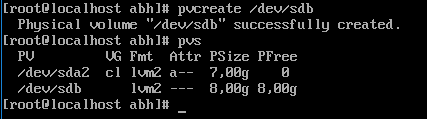
\includegraphics[width=0.7\linewidth]{images/d} 

}

\caption{Creación del nuevo volumen físico `sdb` y comprobación de que se ha creado con la orden `pvs`.}\label{fig:d}
\end{figure}

\begin{enumerate}
\def\labelenumi{\arabic{enumi}.}
\setcounter{enumi}{4}
\tightlist
\item
  Ahora hay que extender el Grupo de Volúmenes (VG) llamado \texttt{cl} con este nuevo volumen físico (recordemos la jerarquía de particiones y nomenclatura que establecía LVM) mediante la orden \texttt{vgextend}, y comprobamos que lo hemos hecho bien en la figura \ref{fig:e}.
\end{enumerate}

\begin{figure}

{\centering 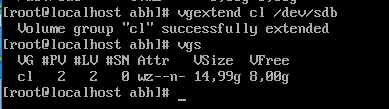
\includegraphics[width=0.7\linewidth]{images/e} 

}

\caption{Extendiendo el grupo de volúmenes `cl` y comprobando que lo hemos hecho bien con el comando `vgs`.}\label{fig:e}
\end{figure}

Y vemos que ya el campo \texttt{\#PV} aparece con el valor \texttt{2}.

\begin{enumerate}
\def\labelenumi{\arabic{enumi}.}
\setcounter{enumi}{5}
\tightlist
\item
  Ahora vamos a \textbf{crear el nuevo volumen lógico} donde almacenar los datos que queremos, y que montaremos en \texttt{/var} (ver figura \ref{fig:f}):
\end{enumerate}

\begin{figure}

{\centering 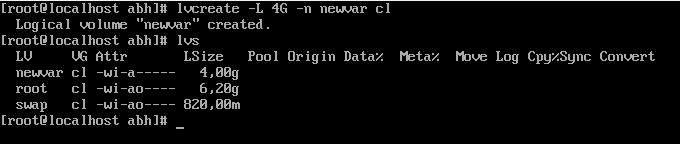
\includegraphics[width=0.9\linewidth]{images/f} 

}

\caption{Creación del volumen lógico con la orden `lvcreate`.}\label{fig:f}
\end{figure}

Y queda comprobado que se ha creado bien.

\begin{enumerate}
\def\labelenumi{\arabic{enumi}.}
\setcounter{enumi}{6}
\tightlist
\item
  Ahora vamos a asignarle un \textbf{sistema de ficheros} mediante el comando \texttt{mkfs} con la opción \texttt{–t} para indicarle el tipo de Sistema de Archivos que le vamos a dar (en este caso, \emph{ext4}), tal y como se muestra en la figura \ref{fig:g}.
\end{enumerate}

\begin{figure}

{\centering 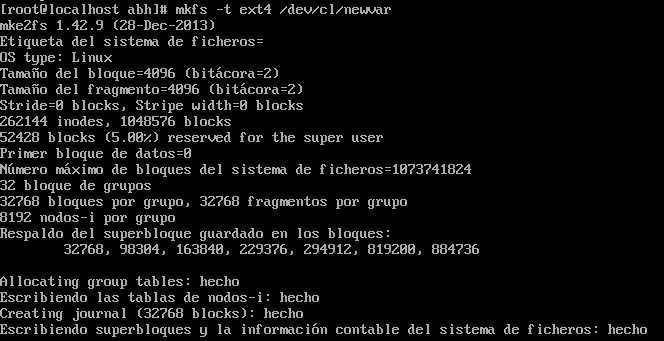
\includegraphics[width=0.8\linewidth]{images/g} 

}

\caption{Asignando un sistema de archivos al nuevo volumen lógico.}\label{fig:g}
\end{figure}

\begin{enumerate}
\def\labelenumi{\arabic{enumi}.}
\setcounter{enumi}{7}
\tightlist
\item
  A continuación, tenemos que \textbf{montar el volumen lógico \texttt{newvar} para que esté accesible}\footnote{Una analogía para recordar por qué montar un volumen: cuando conectamos una unidad de almacenamiento o un lector de DVD, el sistema tiene que crearle lo que se denomina un punto de montaje para poderlo utilizar. Este punto de montaje en casos de discos duros y pendrive's, suele ser una carpeta que creamos manualmente en el sistema o nos lo crea él mismo automáticamente en una partición denominada \texttt{/media} en distribuciones basadas en Ubuntu. En nuestro caso, directamente las montamos sobre \texttt{/mnt/\textless{}dir\_pto\_montaje\textgreater{}}.} sobre un punto de montaje que vamos a crearnos y que se va a llamar \texttt{/mnt/newvar}:
\end{enumerate}

\begin{verbatim}
mkdir /mnt/newvar                           # crear carpeta aux. ` 
mount /dev/cl/newvar /mnt/newvar            # montar VL en aux.
\end{verbatim}

\begin{enumerate}
\def\labelenumi{\arabic{enumi}.}
\setcounter{enumi}{8}
\tightlist
\item
  Vamos a comprobar que el montaje ha sido satisfactorio. Para ello volvemos a ejecutar \texttt{mount} pero sin ninguna opción (o bien con \texttt{\$\ mount\ \textbar{}\ grep\ var}, para que marque en color donde está \texttt{/var}), y en la última línea debería aparecer nuestro dispositivo newvar montado sobre \texttt{/mnt/newvar}, tal y como se muestra en la figura \ref{fig:h}.
\end{enumerate}

\begin{figure}

{\centering 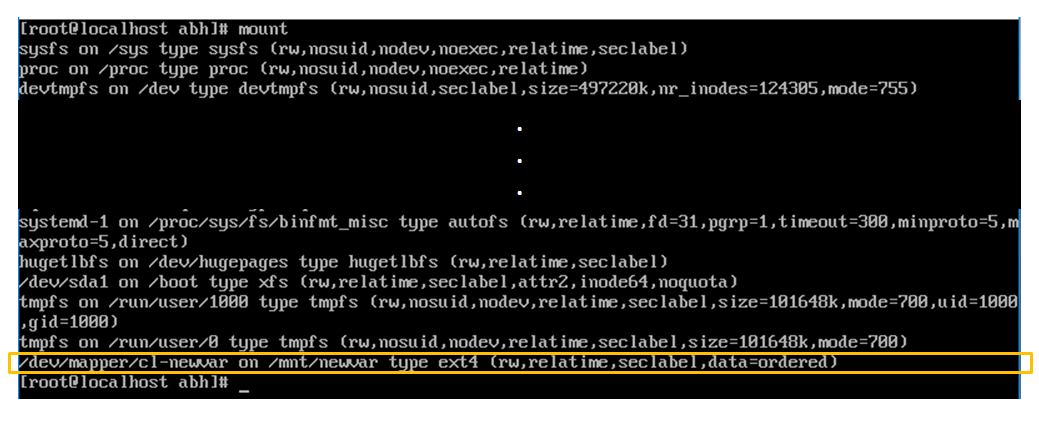
\includegraphics[width=0.8\linewidth]{images/h} 

}

\caption{Fragmento (inicio y fin) de la orden `mount` tras montar newvar sobre el directorio auxiliar `/mnt/newvar` recién creado.}\label{fig:h}
\end{figure}

\begin{enumerate}
\def\labelenumi{\arabic{enumi}.}
\setcounter{enumi}{9}
\tightlist
\item
  Ahora habría que copiar el contenido de /var, que es lo que queremos ampliar, en \texttt{/mnt/newvar}. Pero para evitar que otros usuarios hagan operaciones \emph{r/w} mientras se hace esto, vamos a hacerlo de manera atómica, usando el modo \textbf{AISLADO}. Para ello, ejecutamos el comando
\end{enumerate}

\begin{verbatim}
systemctl isolate runlevel1.target
\end{verbatim}

y tras autenticarnos (con usuario \texttt{root}) debe de aparecer lo mismo que en la figura \ref{fig:i}

\begin{figure}

{\centering 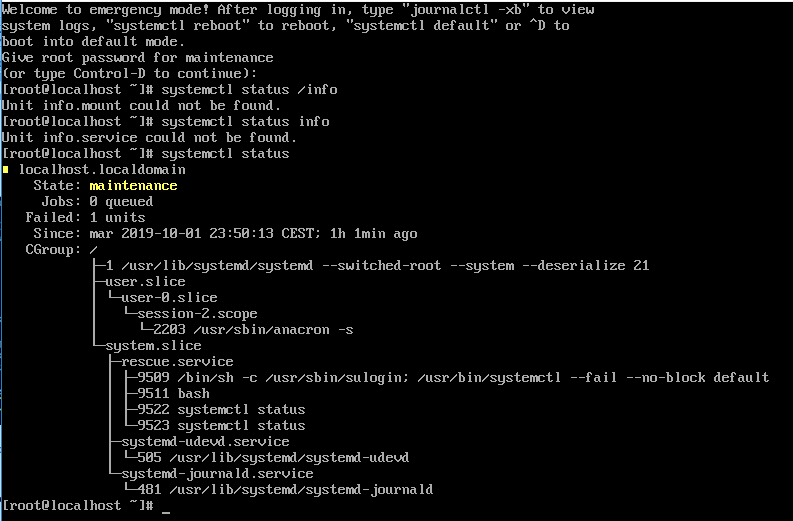
\includegraphics[width=0.8\linewidth]{images/i} 

}

\caption{Aspecto inicial del modo de mantenimiento (modo aislado).}\label{fig:i}
\end{figure}

\hypertarget{literature}{%
\chapter{Literature}\label{literature}}

Here is a review of existing methods.

\hypertarget{methods}{%
\chapter{Methods}\label{methods}}

We describe our methods in this chapter.

\hypertarget{applications}{%
\chapter{Applications}\label{applications}}

Some \emph{significant} applications are demonstrated in this chapter.

\hypertarget{example-one}{%
\section{Example one}\label{example-one}}

\hypertarget{example-two}{%
\section{Example two}\label{example-two}}

\hypertarget{final-words}{%
\chapter{Final Words}\label{final-words}}

We have finished a nice book.

  \bibliography{book.bib,packages.bib}

\end{document}
